\documentclass[11pt,a4paper]{article}
\usepackage[margin=2.35cm]{geometry}
\usepackage{booktabs,graphicx,amsmath,float}
\usepackage[round,authoryear]{natbib}
\usepackage[hidelinks]{hyperref}
\usepackage{fancyhdr}
\graphicspath{{../figures/}}
\pagestyle{fancy}
\fancyhf{}
\fancyhead[L]{\small DSA5205 Project 2}
\fancyhead[R]{\small Group 45}
\fancyfoot[C]{\thepage}
\setlength{\headheight}{14pt}
\setlength{\parindent}{0pt}
\setlength{\parskip}{0.55em}
\setcounter{tocdepth}{1}
\newcommand{\rfzero}{\(r_f=0\)}

\begin{document}
\begin{titlepage}
\centering
\vspace*{2.5cm}
{\large National University of Singapore\par}
\vspace{0.3cm}
{\large DSA5205: Data Science for Quantitative Finance\par}
\vspace{2.2cm}
{\LARGE\bfseries Ridge-Based Monthly Equity Selection\par}
\vspace{0.7cm}
{\Large A validation-led comparison and a test of a momentum-screened portfolio\par}
\vspace{1.8cm}
{\large Project 2 \quad Group 45\par}
\vspace{1cm}
\begin{tabular}{cll}
\toprule
Member & Full name & Student ID \\
\midrule
1 & CHEN HONGXING & \rule{3cm}{0.35pt} \\
2 & LIU WEIYE & \rule{3cm}{0.35pt} \\
3 & WANG KE & \rule{3cm}{0.35pt} \\
4 & ZHAO XIAYU & \rule{3cm}{0.35pt} \\
\bottomrule
\end{tabular}
\vfill
Monthly decisions \quad Next-open execution \quad 20 bps per traded side
\end{titlepage}
\setcounter{page}{2}

\section*{Abstract}
We test whether combining historical signals with Ridge regression improves stock selection within a momentum--volatility screen. Four models share a 30-stock candidate panel, 15 predictors, an adjusted-open return target and the same trading rule. We compared four models on the 2020--2021 validation set. Among the four models, LASSO had the lowest MSE and highest Sharpe. Ridge had the highest Rank IC. We selected Ridge for its validation ranking and its L2 treatment of correlated features. Validation MSE selected \(\alpha=1{,}000\) within Ridge.

The test covers 48 monthly decisions in 2022--2025. Ridge earns a net CAGR of 43.04\% and a Sharpe ratio of 1.272, with \rfzero. Pure momentum within the same screen earns 51.51\% and a Sharpe ratio of 1.590. Ridge exceeds the SPY and QQQ buy-and-hold benchmarks in this sample.

\tableofcontents
\clearpage

\section{Research question and market}
\label{sec:market}
Can a regularised combination of historical signals improve on a simple momentum ranking within a fixed equity universe? Momentum offers a clear benchmark. Gradual incorporation of information can produce continuation over medium horizons \citep{jegadeesh1993}. Shorter-horizon returns, volatility, trend and liquidity describe different market conditions that may help order the candidates. The strategy tests that hypothesis with a monthly portfolio.

We trade US large-cap equities, use US dollars and take the last observed SPY session of each month as the decision date. The signal uses data through that session's close. Positions are established at the next session's open and held until the next rebalance open. SPY and QQQ provide liquid buy-and-hold benchmarks.

\subsection{Data and corporate actions}
We download daily prices, volume and corporate actions from Yahoo Finance using \texttt{yfinance}. The S\&P 500 constituent list comes from Wikipedia. The price used in return calculations is the vendor-adjusted open, computed as the observed open multiplied by the ratio of adjusted close to close. Applying the same convention to stock and ETF returns reflects split and dividend adjustments on both sides of the comparison.

The downloaded universe is a snapshot of current constituents backfilled through time. It omits former members that are absent from the snapshot and includes some firms before they entered the index. Historical active returns therefore depend on the available survivor sample.

\clearpage
\section{Candidate screen and benchmarks}
The screen starts with stocks that close at or above \$5, have at least \$10 million of average daily dollar volume over 20 sessions, meet 95\% price-coverage requirements over 21, 63 and 252 sessions, and have finite values for all predictors. The 300 most liquid eligible names by dollar volume form the broad candidate universe.

We split those names into high, middle and low momentum groups using 12--1 momentum. Within each group, we sort stocks on 63-session realised volatility and take three from the low-volatility cell, four from the middle cell and three from the high-volatility cell. For each cell, the high-momentum group takes the strongest momentum names, the low group takes the weakest, and the middle group takes the names closest to the cell median. Ticker order breaks ties. The symmetric 3--4--3 allocation yields 30 names per decision date.

\begin{table}[H]
\centering
\small
\setlength{\tabcolsep}{4pt}
\begin{tabular}{@{}llp{7cm}l@{}}
\toprule
Portfolio & Role & Selection rule & Weighting \\
\midrule
Ridge & Candidate model & Top 10 Ridge scores in the screened pool & Equal 10\% \\
LASSO & Candidate model & Top 10 LASSO scores in the screened pool & Equal 10\% \\
Random Forest & Candidate model & Top 10 Random Forest scores in the screened pool & Equal 10\% \\
XGBoost & Candidate model & Top 10 XGBoost scores in the screened pool & Equal 10\% \\
\midrule
B1 & Momentum benchmark & Top 10 by 12--1 momentum in the full liquid pool & Equal 10\% \\
B3 & Momentum benchmark & Top 10 by 12--1 momentum in the screened pool & Equal 10\% \\
SPY & ETF benchmark & Buy and hold the S\&P 500 ETF & Fully invested \\
QQQ & ETF benchmark & Buy and hold the Nasdaq-100 ETF & Fully invested \\
\bottomrule
\end{tabular}
\caption{Candidate portfolios and fixed benchmarks.}
\label{tab:strategies}
\end{table}

B3 uses the same screened candidates, weights, trade timing and fees as the model portfolios. This comparison isolates the ranking signal. B1 asks how the active strategy compares with momentum drawn from the broader liquid universe. The ETF comparison describes performance relative to buy-and-hold alternatives.

\clearpage
\section{Target, features and preprocessing}
\label{sec:features}
For a stock selected at decision date \(t\), the label is the adjusted-open simple return
\[
y_{i,t} = \frac{P^{\mathrm{adj,open}}_{i,\mathrm{next\ rebalance}}}
                  {P^{\mathrm{adj,open}}_{i,\mathrm{entry}}}-1.
\]
Here the entry is the next session open after the month-end decision. Each row has a decision date, execution date and label end date in that order. The feature panel uses only information available at the decision close.

\begin{table}[H]
\centering
\footnotesize
\begin{tabular}{p{2.1cm}p{2.8cm}p{5.3cm}p{3.9cm}}
\toprule
Group & Feature & Definition and lookback & Interpretation \\
\midrule
Momentum & mom\_21 & 21-session total return & Short-horizon continuation or reversal \\
Momentum & mom\_63 & 63-session total return & Quarterly momentum \\
Momentum & mom\_126 & 126-session total return & Semi-annual momentum \\
Momentum & mom\_2\_12 & 12-month return, skipping the last month & Classic 12--1 momentum \\
Momentum & relative\_mom\_63 & 63-session return minus SPY return & Relative strength \\
Volatility/risk & vol\_21 & Annualised 21-session realised volatility & Short-term risk \\
Volatility/risk & vol\_63 & Annualised 63-session realised volatility & Screening volatility \\
Volatility/risk & beta\_252 & 252-session rolling beta to SPY & Systematic exposure \\
Volatility/risk & drawdown\_63 & Price relative to 63-session high & Recent loss state \\
Trend & ma\_ratio\_50 & Price relative to 50-session moving average & Short-term trend \\
Trend & ma\_ratio\_200 & Price relative to 200-session moving average & Long-term trend \\
Trend & rsi\_14 & 14-session relative strength index & Overbought/oversold \\
Liquidity & ln\_adv\_20 & Log 20-session average dollar volume & Size and liquidity \\
Liquidity & volume\_ratio\_21 & Volume relative to 21-session average & Abnormal activity \\
Range & range\_hl & High--low range scaled by close & Intraday price pressure \\
\bottomrule
\end{tabular}
\caption{The fifteen predictors, grouped by economic mechanism. All inputs are available at the month-end decision close.}
\label{tab:features}
\end{table}


Short, intermediate and long lookbacks allow the model to use several horizons of momentum and trend. The 12--1 feature omits the most recent month to distinguish medium-horizon continuation from short-horizon reversal. Relative momentum measures the stock's return in excess of SPY over the same lookback. The volatility and risk features measure recent dispersion, market sensitivity and drawdown.

Candidate rows require finite features. Auxiliary features can be carried forward for at most two sessions. The screening variables use observations at the decision date. Ridge and LASSO scale inputs using a standardiser fitted with the respective training rows. The tree models use the original feature scales.

\clearpage
\section{Models and control of overfitting}
\label{sec:model}
The 15 features fall into five economic groups. Several measure related effects at different horizons. For example, 63-session momentum and its market-relative version have a training correlation of 0.939. The correlation between 126-session momentum and the 200-session moving-average ratio is 0.936. Appendix~\ref{app:diagnostics} reports the training-period correlations.

Ridge gives the related predictors a joint linear score. It fits an intercept \(b\) and penalises the squared coefficient norm \citep{hoerl1970}
\[
(\hat b,\hat\beta)
=\arg\min_{b,\beta}\left\{
\sum_i (y_i-b-x_i^\top\beta)^2 + \alpha\sum_j\beta_j^2
\right\}.
\]
The penalty reduces the influence of weak predictors and helps control coefficient variation when predictors move together.  LASSO applies an L1 penalty, which can set some coefficients exactly to zero \citep{tibshirani1996}. Random Forest averages regression trees. XGBoost fits a sequence of regularised trees. The tree models allow nonlinear effects and interactions.

\begin{table}[H]
\centering
\begin{tabular}{lp{8.7cm}r}
\toprule
Model & Grid & Count \\
\midrule
Ridge & \(\alpha\in\{0.1,1,10,100,1000,10000\}\) & 6 \\
LASSO & \(\alpha\in\{10^{-5},10^{-4},10^{-3},10^{-2},10^{-1}\}\) & 5 \\
Random Forest & Depth 3 or 6, minimum leaf size 10 or 25 & 4 \\
XGBoost & Depth 2 or 3, learning rate 0.03 or 0.10, 100 or 200 trees & 8 \\
\bottomrule
\end{tabular}
\caption{The 23 configurations evaluated on validation.}
\label{tab:grid}
\end{table}

Random Forest uses 250 trees and a feature fraction of 0.7. XGBoost uses row and column fractions of 0.8 and an L2 tree penalty of 10. Model training uses seed 42 where applicable. Holding the grid and split fixed limits the search and makes the four model families comparable.

\clearpage
\section{Chronological split and fitting}
\label{sec:split}
The raw price history starts in 2009, which supplies lookback observations for 2010 decisions. We fixed the training, validation and test date blocks in Table~\ref{tab:split} before fitting the models. A row enters a fitting or validation block when its holding-period return has settled by the corresponding cutoff. The last two decisions of 2019 settle in 2020, and the last two decisions of 2021 settle in 2022. They are excluded from the affected blocks.

\begin{table}[H]
\centering
\begin{tabular}{llrrl}
\toprule
Use & Decision years & Months & Rows & Last label end \\
\midrule
Train each configuration & 2010--2019 & 118 & 3,540 & 2 Dec 2019 \\
Compare configurations & 2020--2021 & 22 & 660 & 1 Dec 2021 \\
Refit selected model & 2010--2021 & 142 & 4,260 & 1 Dec 2021 \\
Test selected model & 2022--2025 & 48 & 1,440 & 2 Feb 2026 \\
\bottomrule
\end{tabular}
\caption{Eligible observations after applying the realised-label cutoff. Each decision month contains 30 candidates.}
\label{tab:split}
\end{table}

For the validation comparison, each configuration is fitted on the same eligible training rows. We estimate linear-model scaling parameters with those rows and apply the fitted transformation to validation features. Within each family, the selected configuration is the one with the lowest validation MSE.

After model selection, we refit the selected model and its preprocessing on the eligible observations through 2021. The fitted model stays fixed across the 48 test decisions.

\clearpage
\section{Validation and choice of Ridge}
\label{sec:validation}
We compared the four selected configurations and the fixed benchmarks over the same 22 validation decisions. All four models used the same 30 candidates and equal-weight Top-10 rule. MSE measures error in predicted return levels. Rank IC averages the monthly Spearman correlations between scores and realised returns across all 30 candidates. The models use predicted returns as scores, and B3 uses momentum. Validation Sharpe uses net monthly returns and \rfzero.

\begin{table}[H]
\centering
\begin{tabular}{lrrrr}
\toprule
Strategy & MSE & Rank IC & Net CAGR & Sharpe \\
\midrule
Ridge & 0.022422 & \textbf{0.0438} & 45.69\% & 0.918 \\
LASSO & \textbf{0.022281} & 0.0250 & 46.14\% & 0.926 \\
Random Forest & 0.022412 & 0.0261 & 40.20\% & 0.866 \\
XGBoost & 0.022642 & -0.0098 & 26.59\% & 0.693 \\
\midrule
B1 & --- & --- & 64.13\% & 1.341 \\
B3 & --- & 0.0332 & 38.41\% & 1.074 \\
SPY & --- & --- & 23.17\% & 1.048 \\
QQQ & --- & --- & 38.72\% & 1.566 \\
\bottomrule
\end{tabular}
\caption{Post-cost validation results over the same 22 monthly decisions. Sharpe uses a zero risk-free rate.}
\label{tab:validation}
\end{table}


B3 earned a validation Sharpe of 1.074 versus 0.918 for Ridge. Ridge had higher net CAGR over those dates, at 45.69\% versus 38.41\% for B3.

Among the four models, LASSO had the lowest validation MSE and highest Sharpe. Its selected fit set six of the 15 coefficients to zero. Ridge had the highest validation Rank IC (0.0438), with an MSE 0.63\% higher than LASSO's. We selected Ridge for its cross-sectional ranking accuracy and its use of L2 shrinkage to combine related predictors across five feature groups.

Within Ridge, validation MSE selected \(\alpha=1{,}000\). We refitted that specification on the eligible pre-test observations and evaluated it against the fixed benchmarks in 2022--2025.

\clearpage
\section{From forecasts to trades}
\label{sec:trades}
At each month-end, Ridge scores the 30 eligible stocks. We rank them by predicted return, break score ties by ticker, and assign 10\% target weight to each of the ten highest-ranked stocks. The remaining targets are zero. The portfolio is fully invested, long-only and unlevered. Figure~\ref{fig:position} shows the scores and positions for one decision date.

\begin{figure}[H]
\centering
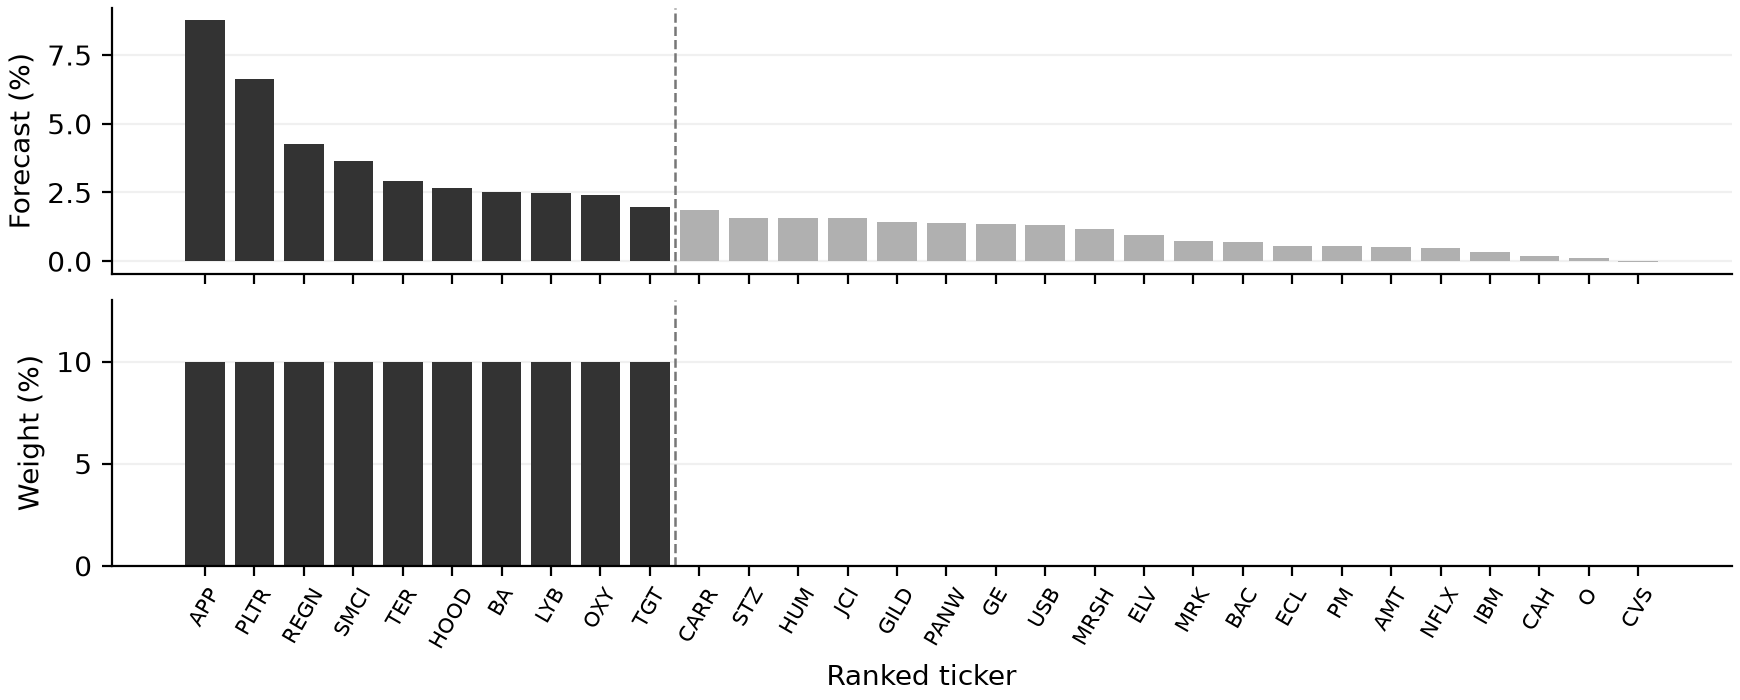
\includegraphics[width=0.94\textwidth]{fig_score_to_position.png}
\caption{Ridge scores and equal weights for the 30 June 2025 decision.}
\label{fig:position}
\end{figure}

Weights drift with stock returns before the next rebalance. If \(w^{\mathrm{target}}_{i,t}\) and \(w^{\mathrm{pre}}_{i,t}\) are the new and drifted weights, the fee is
\[
c_t=0.002\sum_i |w^{\mathrm{target}}_{i,t}-w^{\mathrm{pre}}_{i,t}|.
\]
We subtract it from the gross holding-period return. The initial purchase charges one side. Later rebalances charge the changes in exposure. B1 and B3 use the same cost calculation. SPY and QQQ each incur a single entry fee.

\clearpage
\section{Ridge forecasts on the test period}
\label{sec:forecast}
The test spans 48 monthly decisions from 31 January 2022 to 31 December 2025. Actual holding starts on 1 February 2022 and ends on 2 February 2026. Consecutive holding periods meet at the next rebalance open.

\begin{table}[H]
\centering
\begin{tabular}{lr}
\toprule
Forecast metric & Ridge \\
\midrule
Observations & 1,440 \\
MSE & 0.015057 \\
MAE & 0.082802 \\
Mean monthly Rank IC & 0.0619 \\
Months with positive Rank IC & 56.25\% \\
Out-of-sample \(R^2\) & 0.0187 \\
\bottomrule
\end{tabular}
\caption{Forecast performance on the 30-stock test panel.}
\end{table}

For the benchmark-relative \(R^2\), we compare the model's error with a constant forecast given by the mean return of the eligible pre-test refit sample \citep{campbell2008}. The score is \(1-\mathrm{SSE}_{\mathrm{Ridge}}/\mathrm{SSE}_{\mathrm{mean}}\). Ridge reduces squared error by approximately 1.87\% relative to that forecast. The average Rank IC is positive. These metrics describe forecast performance on all candidates. The portfolio evaluation measures what the top ten scores earn after costs.

\begin{figure}[H]
\centering
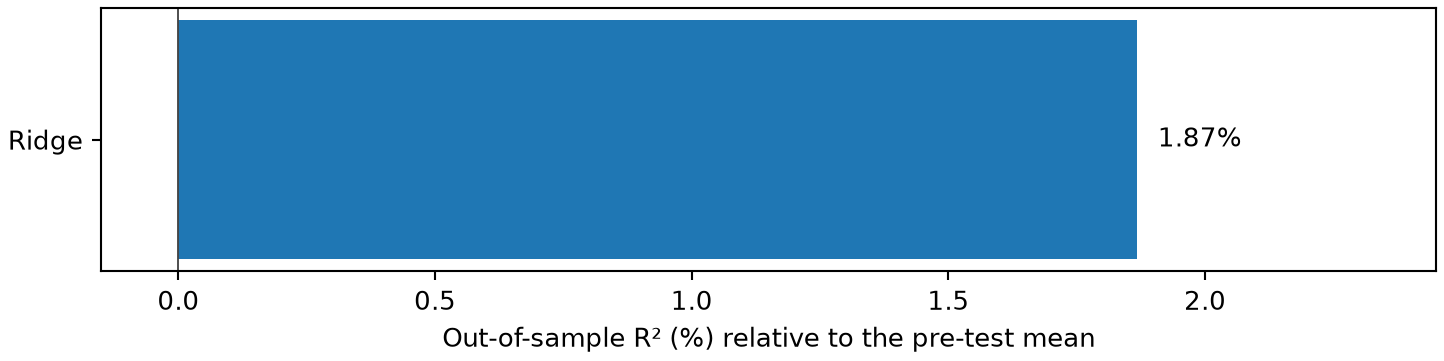
\includegraphics[width=0.9\textwidth]{ridge_oos_r2.png}
\caption{Test-period forecast improvement against the historical-mean predictor.}
\end{figure}

\clearpage
\section{Ridge portfolio and benchmark results}
\label{sec:performance}
\begin{table}[H]
\centering
\begin{tabular}{lrrrrr}
\toprule
Strategy & Net CAGR & Volatility & Sharpe & Max drawdown & Turnover \\
\midrule
Ridge & 43.04\% & 32.56\% & 1.272 & -28.54\% & 1.26 \\
B1 & 73.13\% & 37.72\% & 1.664 & -19.19\% & 0.65 \\
B3 & 51.51\% & 29.04\% & 1.590 & -14.99\% & 0.94 \\
SPY & 12.72\% & 15.27\% & 0.863 & -19.67\% & 0.02 \\
QQQ & 14.81\% & 19.93\% & 0.796 & -25.56\% & 0.02 \\
\bottomrule
\end{tabular}
\caption{Post-cost test results for Ridge and the four fixed benchmarks. CAGR, volatility and Sharpe are annualised. Turnover is the average monthly sum of absolute weight changes.}
\label{tab:oos}
\end{table}


Ridge compounds to 4.19 times its initial value after costs. It exceeds SPY and QQQ on CAGR and Sharpe, with higher annualised volatility. B3 is the direct benchmark for stock ranking. B3 exceeds Ridge by 8.47 percentage points of CAGR and 0.318 of Sharpe, and has lower turnover and a shallower period-end drawdown.

\begin{figure}[H]
\centering
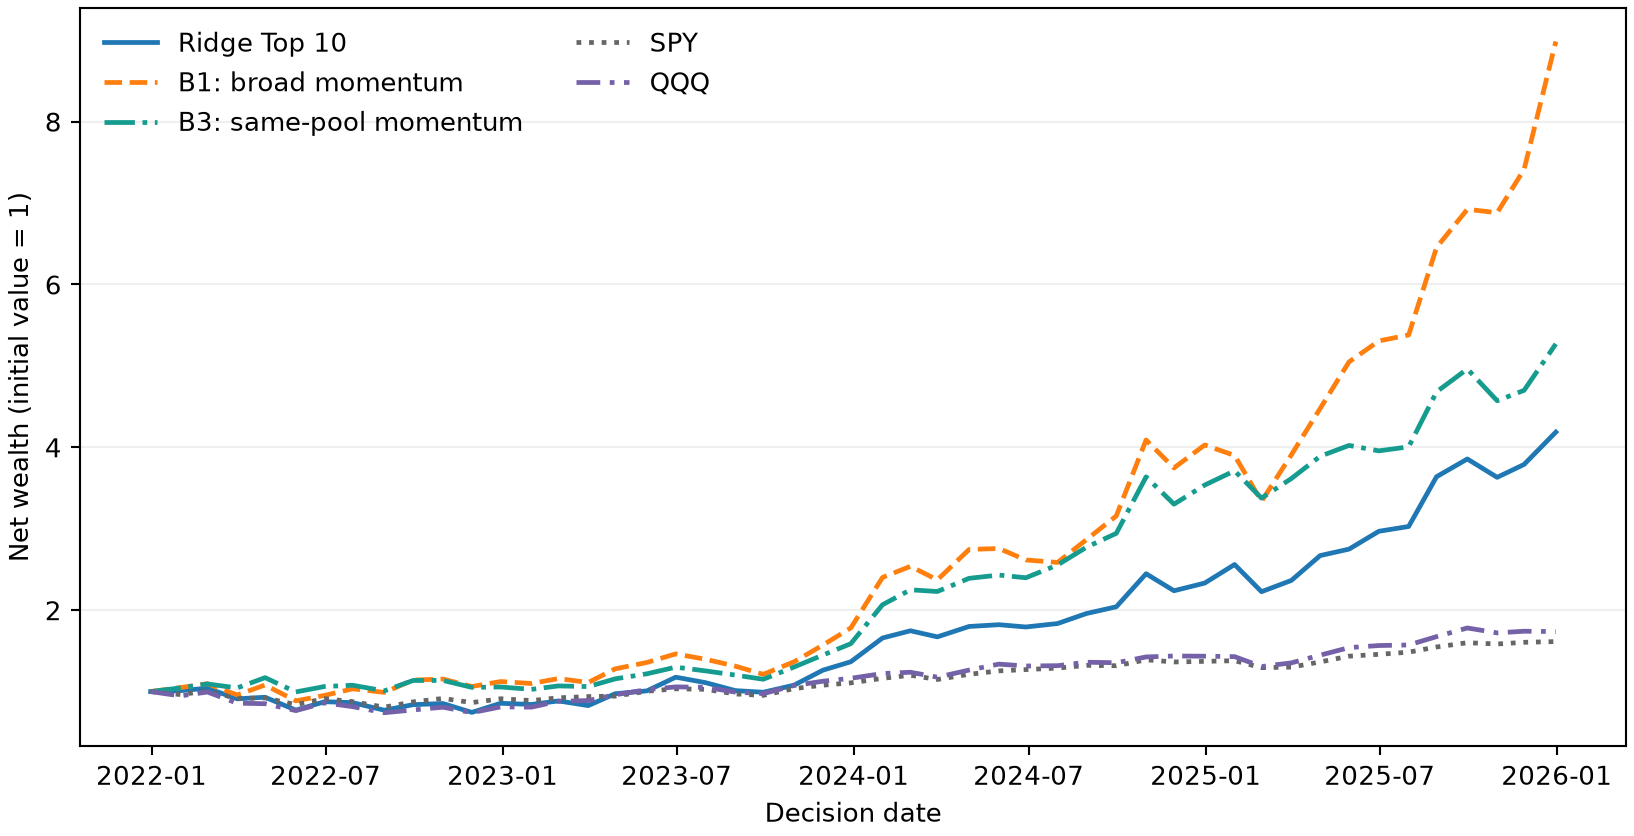
\includegraphics[width=0.95\textwidth]{ridge_benchmarks.png}
\caption{Cumulative net wealth, indexed to the decisions that initiated each holding period.}
\label{fig:wealth}
\end{figure}

Ridge's gross CAGR is 47.30\%. Costs reduce it to 43.04\%, a difference of 4.26 percentage points. Average monthly two-way turnover is 1.26, compared with 0.94 for B3 and 0.65 for B1. Sharpe ratios use a zero risk-free rate \citep{sharpe1966}. Drawdown uses rebalance-period wealth.

\clearpage
\section{Performance by decision year}
\label{sec:year}
Annual cohorts group returns by the year of the decision date. The holding period associated with a December decision is implemented in the following year. Each cohort contains 12 decisions. The yearly Sharpe estimates use the monthly returns in each cohort and the same annualisation and risk-free conventions as the full-period comparison.

\begin{table}[H]
\centering
\begin{tabular}{lrrrrr}
\toprule
Decision year & Ridge & B1 & B3 & SPY & QQQ \\
\midrule
2022 & -14.36\% & 12.33\% & 5.63\% & -8.82\% & -18.79\% \\
2023 & 59.52\% & 58.61\% & 50.35\% & 21.42\% & 43.23\% \\
2024 & 70.77\% & 126.14\% & 122.68\% & 23.86\% & 23.34\% \\
2025 & 79.47\% & 122.99\% & 49.00\% & 17.72\% & 21.10\% \\
\bottomrule
\end{tabular}
\caption{Net compound returns by decision year.}
\label{tab:annual}
\end{table}

\begin{figure}[H]
\centering
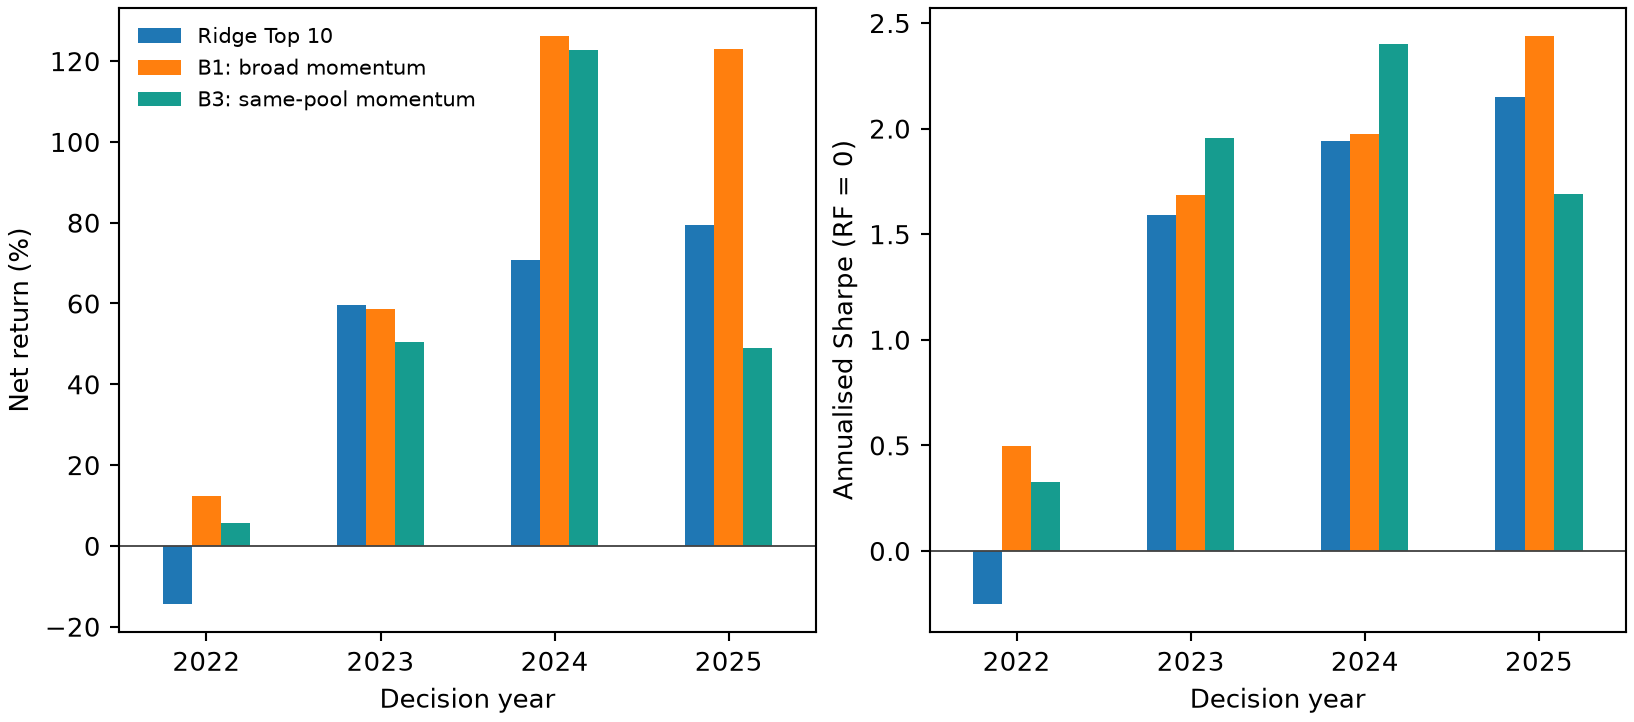
\includegraphics[width=0.96\textwidth]{annual_returns_sharpe.png}
\caption{Net returns and Sharpe ratios by decision-year cohort.}
\end{figure}

Ridge earns a higher net return than B3 in 2023 and 2025. B3 has the higher Sharpe in three of the four years. The largest net return gap is in 2024, when B3 earns 122.68\% and Ridge earns 70.77\%. In 2022, Ridge loses 14.36\% while B3 gains 5.63\%.

\clearpage
\section{Interpretation and limitations}
\label{sec:interpret}
\paragraph{Forecast and portfolio outcomes.}
Ridge improved on the historical-mean forecast and the portfolio earned a higher CAGR than SPY and QQQ. B3 used the same candidates, weights and execution rule and achieved higher net CAGR and Sharpe with lower turnover. The same-pool comparison favours momentum over Ridge for stock selection in this sample.

\paragraph{Market exposure.}
A regression on SPY using 48 monthly observations gives Ridge a beta of 1.64 and an annualised single-factor intercept of 21.73\%, with a zero risk-free rate.

\paragraph{Stock universe.}
Backfilling current index constituents excludes former members and includes some stocks before they joined. This affects how we interpret returns for both the Ridge and momentum portfolios.

\clearpage
\section{Reproducibility and contributions}
\label{sec:repro}
The monthly study uses the packaged derived panels and the following commands from the project root.
\begin{verbatim}
python -m pip install -r requirements.txt
python run_primary_study.py
\end{verbatim}
The notebook runs the same workflow. The \texttt{--rebuild-data} flag regenerates the monthly panels from Yahoo Finance and the current constituent list.

\begin{table}[H]
\centering
\begin{tabular}{lp{7.8cm}}
\toprule
Location & Contents \\
\midrule
\texttt{config/experiment\_config.yaml} & Dates, seed, model grids and portfolio settings. \\
\texttt{results/validation/} & Validation model and benchmark results, tuning grid and Ridge decision record. \\
\texttt{results/oos/} & Ridge forecasts, benchmark returns, annual results and performance table. \\
\texttt{figures/} & Forecast, portfolio and diagnostic figures. \\
\bottomrule
\end{tabular}
\caption{Reproduction map.}
\end{table}

\subsection*{Member contributions}
\begin{tabular}{lp{10.4cm}}
\toprule
Member & Contribution \\
\midrule
CHEN HONGXING & Proposed the trading strategy, led the candidate screening and stock selection design, and synthesised the benchmark findings. \\
LIU WEIYE & Prepared the market data, constructed features and forward-return labels, and checked the alignment of decision, execution and label dates. \\
WANG KE & Trained and validated the four models, compared hyperparameter settings, and documented the choice of Ridge. \\
ZHAO XIAYU & Ran the backtests with transaction costs, compared performance against the benchmarks, produced the figures and organised the submission files. \\
\bottomrule
\end{tabular}

\subsection*{AI use}
The team used AI assistance for code organisation, drafting and verification of the reporting workflow.

\clearpage
\appendix
\section{Training-period diagnostics}
\label{app:diagnostics}
Twelve of 105 feature pairs have a training-sample absolute correlation of at least 0.70. Figure~\ref{fig:correlation} illustrates how momentum and trend overlap, and how volatility measures move together.

\begin{figure}[H]
\centering
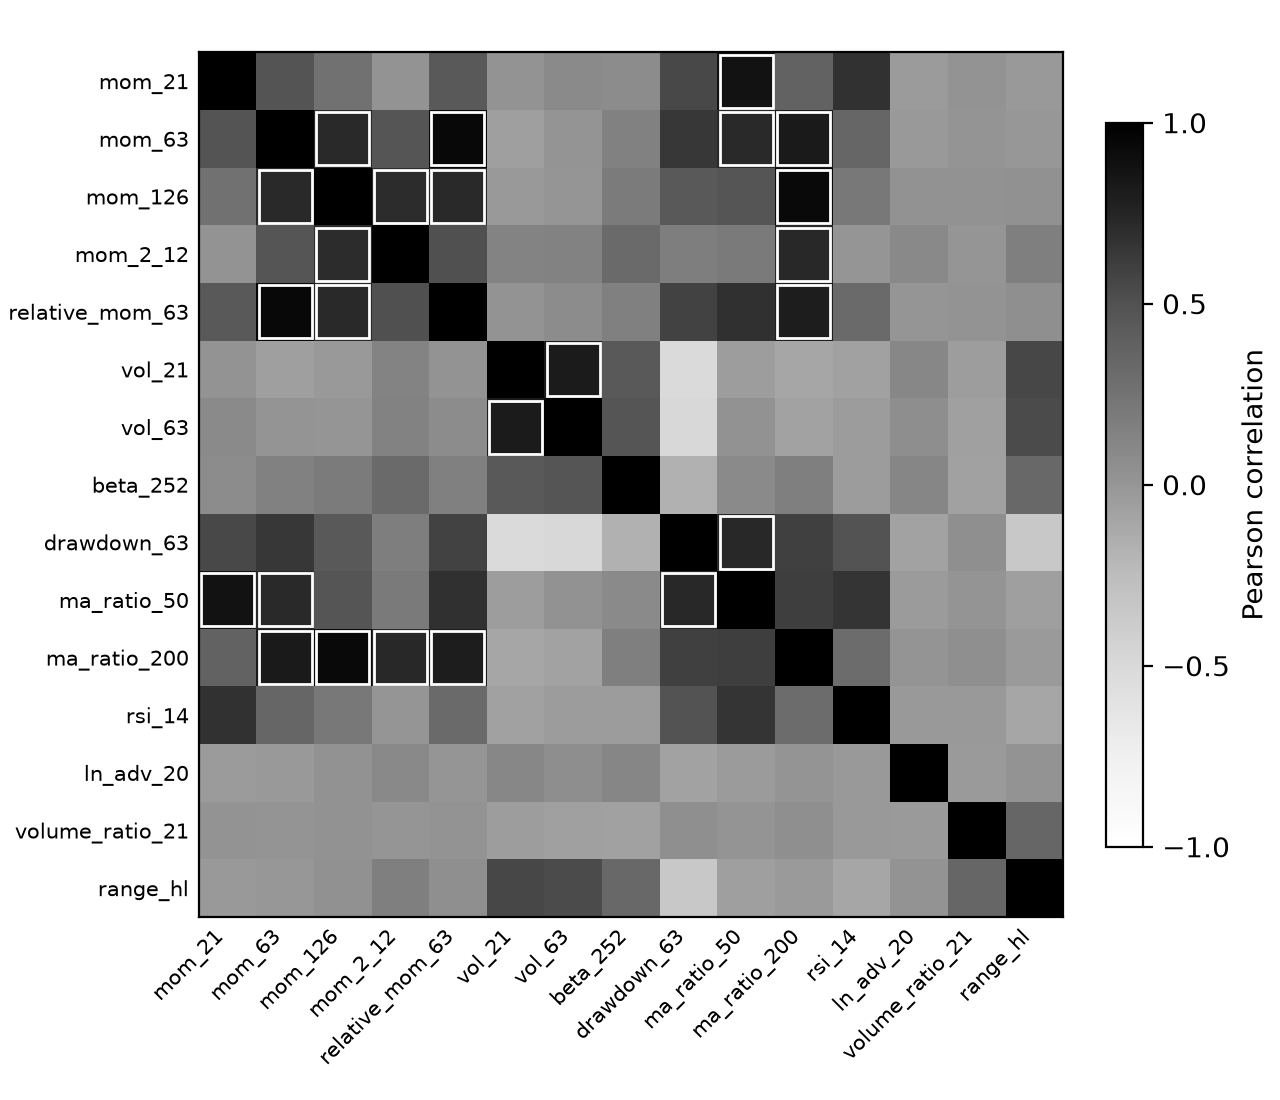
\includegraphics[width=0.68\textwidth]{fig_correlation.png}
\caption{Pearson correlations of the 15 features on the training rows.}
\label{fig:correlation}
\end{figure}

\clearpage
\begin{thebibliography}{9}
\bibitem[Campbell and Thompson(2008)]{campbell2008}
Campbell, J. Y., and S. B. Thompson. 2008.
Predicting excess stock returns out of sample.
\textit{Review of Financial Studies} 21(4), 1509--1531.
\bibitem[Hoerl and Kennard(1970)]{hoerl1970}
Hoerl, A. E., and R. W. Kennard. 1970.
Ridge regression: biased estimation for nonorthogonal problems.
\textit{Technometrics} 12(1), 55--67.
\bibitem[Jegadeesh and Titman(1993)]{jegadeesh1993}
Jegadeesh, N., and S. Titman. 1993.
Returns to buying winners and selling losers: implications for stock market efficiency.
\textit{Journal of Finance} 48(1), 65--91.
\bibitem[Sharpe(1966)]{sharpe1966}
Sharpe, W. F. 1966.
Mutual fund performance. \textit{Journal of Business} 39(1), 119--138.
\bibitem[Tibshirani(1996)]{tibshirani1996}
Tibshirani, R. 1996.
Regression shrinkage and selection via the Lasso.
\textit{Journal of the Royal Statistical Society: Series B} 58(1), 267--288.
\end{thebibliography}
\end{document}
